\documentclass[12pt]{article}

\usepackage{amsmath}
\usepackage{amssymb}
\usepackage[dvips]{graphicx}
\usepackage{eepic}
\usepackage{color}
\usepackage{wasysym} % \female \male
\usepackage[landscape,pdftex]{geometry}
\usepackage{fancyhdr}
\usepackage{hyperref}

\definecolor{cantelope}{rgb}{1.0,0.8,0.4}
\hypersetup{
    colorlinks, urlcolor={cantelope}
}
\hypersetup{pdfpagemode=UseNone} % don't show bookmarks on initial view

\DeclareOption{bigsym}{\DeclareSymbolFont{largesymbols}{OMX}{psycm}{m}{n}}
\ProcessOptions

\setlength{\oddsidemargin}{-0.75in}
\setlength{\evensidemargin}{-0.75in}
\setlength{\topmargin}{-1in}
\setlength{\textheight}{7.75in}
\setlength{\textwidth}{10.5in}
\setlength{\footskip}{0in}
\setlength{\parindent}{0pt}
\setlength{\rightskip}{0pt plus 1fil} % makes ragged right

\renewcommand{\familydefault}{phv} % helvetica

% following: color
\definecolor{mybgcolor}{rgb}{0,0,0.3125}
\definecolor{myyellow}{rgb}{1,1,0.4}
\definecolor{myblue}{rgb}{0.4,0.8,1}
\definecolor{mypink}{rgb}{1,0.4,1}
\definecolor{mywhite}{rgb}{1,1,1}

% header/footer layout
\pagestyle{fancy}
\lhead{} \chead{} \rhead{}
\lfoot{} \cfoot{} \rfoot{\color{myyellow} \thepage}
\renewcommand{\headrulewidth}{0pt}
\renewcommand{\footrulewidth}{0pt}

% font sizes
\newcommand{\superlarge}{\fontsize{60}{60} \selectfont}
\newcommand{\titlesize}{\fontsize{40}{50} \selectfont}
\newcommand{\headsize}{\fontsize{35}{35} \selectfont}
\newcommand{\textsize}{\fontsize{30}{35} \selectfont}
\newcommand{\smallsize}{\fontsize{25}{30} \selectfont}
\newcommand{\smallersize}{\fontsize{20}{25} \selectfont}
\newcommand{\smallestsize}{\fontsize{18}{22} \selectfont}
\newcommand{\lod}{\text{LOD}}
\newcommand{\plod}{\text{pLOD}}
\newcommand{\bic}{\text{BIC}}
\newcommand{\rss}{\text{RSS}}
\newcommand{\var}{\text{var}}
\newcommand{\M}{\text{M}}


\pagecolor{mybgcolor}
\color{mywhite}

\begin{document}
\thispagestyle{empty}

\begin{center}
\titlesize \color{myyellow}


\vspace*{15mm}

R/qtl2 Workshop

\color{mypink}
\rule{10in}{1mm}

\vspace{5mm}

\textsize \color{myblue}
Karl Broman
\vspace{5mm}

\color{mywhite}
{\smallsize Biostatistics and Medical Informatics

University of Wisconsin -- Madison
\vspace{20mm}


\href{http://kbroman.org/qtl2}{\tt kbroman.org/qtl2} \\[3pt]
\href{http://kbroman.org}{\tt kbroman.org} \\[3pt]
\href{https://github.com/kbroman}{\tt github.com/kbroman} \\
\href{https://twitter.com/kwbroman}{\tt @kwbroman} \\
}

\end{center}

\newpage

\headsize \color{myyellow}
\hfill \begin{minipage}{5.75in}
\centering
Why R/qtl2?
\end{minipage}

\vspace{3cm}

\color{mywhite} \smallsize

\hfill \begin{minipage}[t]{9.5in}
\begin{itemize}
\itemsep24pt
\setlength{\rightskip}{0pt plus 1fil} % makes ragged right
\item High-dimensional data
  \begin{itemize}
  \item[] {\color{myblue} \smallersize genotypes and phenotypes}
  \end{itemize}
\item More diverse crosses
  \begin{itemize}
  \item[] {\color{myblue} \smallersize especially multi-parent populations}
  \end{itemize}
\item Linear mixed models
  \begin{itemize}
  \item[] {\color{myblue} \smallersize especially in DO/HS/AIL}
  \end{itemize}
\end{itemize} \end{minipage}


\newpage

\headsize \color{myyellow}
\hfill\begin{minipage}{5.75in}
\centering
R/qtl $\rightarrow$ R/qtl2
\end{minipage}

\vspace{1cm}

\color{mywhite} \smallsize

\hfill \begin{minipage}[t]{9.5in}
\begin{itemize}
\setlength{\rightskip}{0pt plus 1fil} % makes ragged right
\item See
  \href{http://kbroman.org/qtl2/assets/vignettes/rqtl_diff.html}{\smallestsize
    \tt kbroman.org/qtl2/assets/vignettes/rqtl\_diff.html}
\item New data file formats
\item New data structures
\item Split into multiple packages
  \begin{itemize}
  \item[] {\color{myblue} \smallersize qtl2geno, qtl2scan, qtl2plot, qtl2convert}
  \end{itemize}
\item New function names
  \begin{itemize}
  \item[] {\color{myblue} \smallersize \verb|read.cross()| $\rightarrow$ \verb|read_cross2()|}
  \item[] {\color{myblue} \smallersize \verb|calc.genoprob()| $\rightarrow$ \verb|calc_genoprob()|}
  \item[] {\color{myblue} \smallersize \verb|scanone()| $\rightarrow$ \verb|scan1()|}
  \end{itemize}
\item Different treatment of intermediate calculations
\item Use of individual IDs for aligning data
\item Order of args when subsetting cross objects
  \begin{itemize}
  \item[] {\color{myblue} \smallersize \verb|cross[chr,ind]| $\rightarrow$ \verb|cross2[ind,chr]|}
  \end{itemize}
\end{itemize} \end{minipage}




\newpage

\headsize \color{myyellow}
$\boldsymbol{\rightarrow}$ R

\vspace{3cm}

\color{mywhite} \smallsize

\hfill \begin{minipage}[t]{9.5in}
\begin{itemize}
\itemsep24pt
\item \verb|convert2cross2()|
\item \verb|summary()|, \verb|n_ind()|, \verb|n_mar()|, \dots
\item \verb|insert_pseudomarkers()|
\item \verb|calc_genoprob()|
\item \verb|scan1()|
\item \verb|find_peaks()|
\end{itemize} \end{minipage}


\newpage

\headsize \color{myyellow}
\hfill\begin{minipage}{5.75in}
\centering
Linear mixed models
\end{minipage}


\vspace{3cm}

\color{mywhite} \textsize

$$\begin{array}{lllcl@{\qquad}l}
  y_i & = & \mu + & \textstyle{{\color{mypink} \sum_k \beta_k q_{ik}}} & + \epsilon_i
               & \epsilon_i \sim \text{N}(0, \sigma^2_e) \\[24pt]
  & = & \mu + & {\color{mypink} \eta_i} & + \epsilon_i & \eta_i \sim \text{N}(0, \sigma^2_p)
\end{array}$$

\vspace{2cm}

$$\text{cov}(\eta_i, \eta_j) = \sigma^2_p \; (2 k_{ij})$$



\newpage

\headsize \color{myyellow}
\hfill\begin{minipage}{5.75in}
\centering
DO genotype reconstruction
\end{minipage}

\centerline{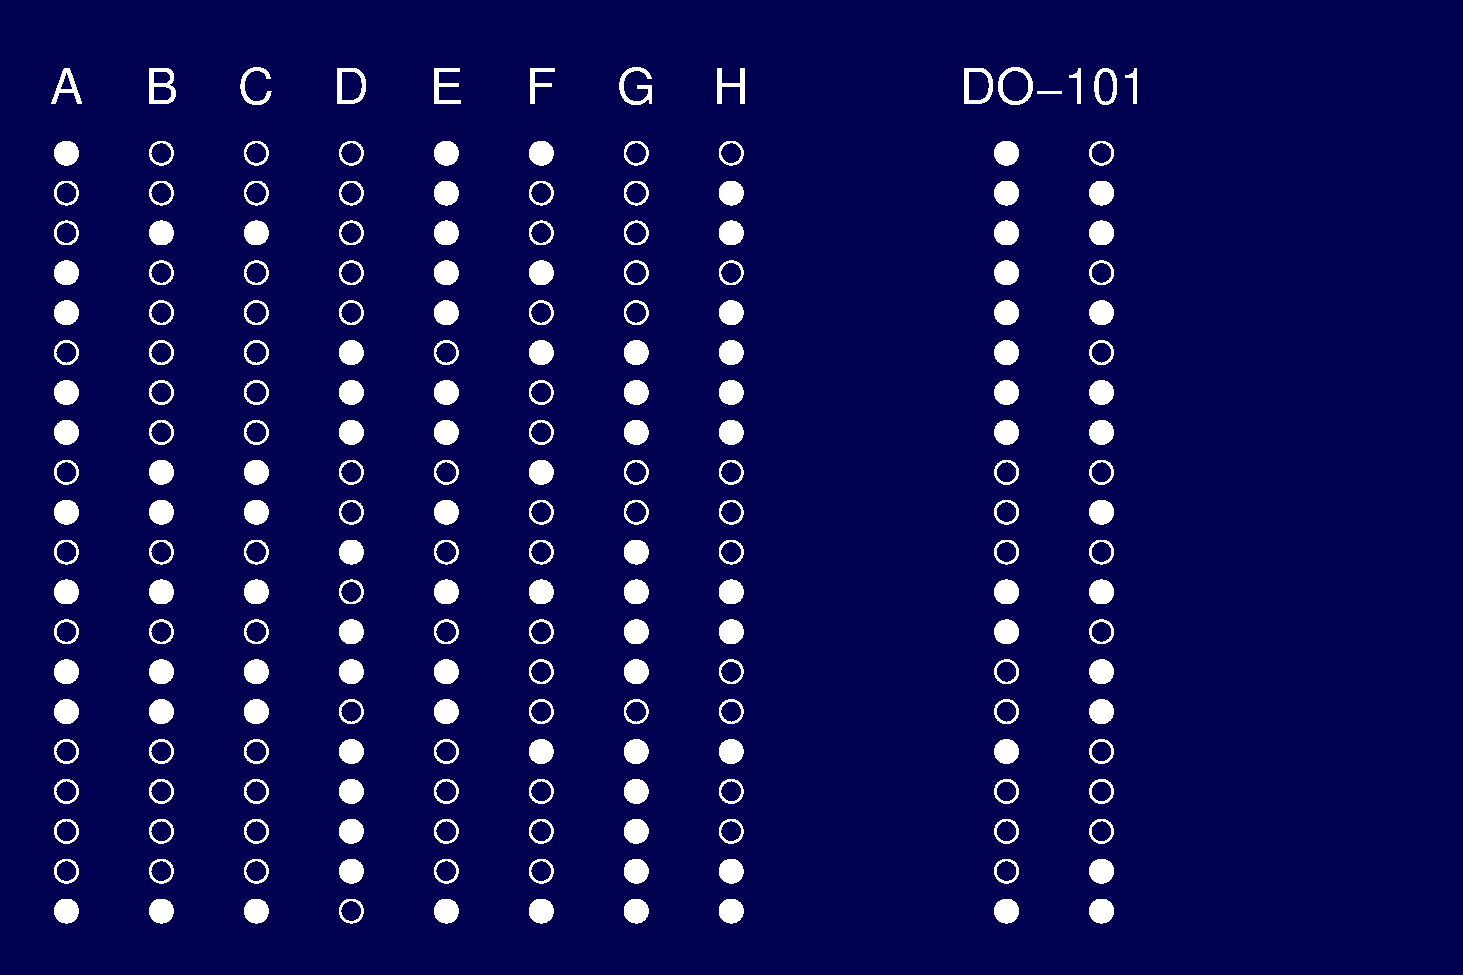
\includegraphics{Figs/genoprobs.pdf}}

\end{document}
